\chapter[Introduction]{Introduction}
\label{ch:intro}
\vspace{-16pt}
\begin{chapquote}{Isaac Asimov} \singlespacing The most exciting phrase to hear in science, the one that heralds discoveries, is not ‘Eureka!’ but ‘Now that’s funny…
\end{chapquote} \vspace{-8pt}
\begin{chapquote}{Brian W. Kernighan} \singlespacing Debugging is twice as hard as writing the code in the first place. Therefore, if you write the code as cleverly as possible, you are, by definition, not smart enough to debug it
\end{chapquote} \vspace{-8pt}

\noindent\makebox[\linewidth]{\rule{0.5\textwidth}{0.5pt}} \vspace{1pt}

\newcommand{\code}{\textsc}
\newcommand{\Hmolecular}{H$_2$}
%\newcommand{\hii}{H\sc{I}}
%\newcommand{\hii}{H{\sc{II}}}

%
% \beq
% \frac{\mathrm{d}}{\mathrm{d}t} \int_S \mathbf{B} \cdot \mathrm{d}S = 0,f
% \eeq
Galaxies are amalgamations of gas and stars embedded in dark matter halos. They are formed over cosmic time as the products of the hierarchical assembly that follows from the collapse of the primordial density fluctuations that arose after the Big Bang. The gravitational pull of dark matter -- as predicted from $\Lambda$CDM cosmology -- controls the hierarchical growth of structure in the Universe. While, broadly speaking, the evolution of baryons is dominated by this pull, the beautiful simplicity of $\Lambda$CDM cosmology is muddied by their existence. The complexities of hydrodynamics, magnetohydrodynamics, thermodynamics, chemistry, radiative processes, and nucleosynthesis -- or, ``astrophysics" for short -- drives these deviations and gives rise to the Universe that we observe. In spite of a concerted effort spanning nearly a century, we are far from a self-consistent theory of galaxy evolution (see \citet{SomervilleDave2015} and \cite{NaabOstriker2017} for recent reviews). It is understanding the rich set of physics that formed our own Galaxy and the countless galaxies scattered throughout the Universe that motivates this work.

A substantial slice of modern astrophysics has been devoted towards understanding the chemical evolution -- the abundances of individual elements in space and time -- of the Universe. With the exception of H, He, and trace amounts of light elements, all of the elements in the Universe are produced in nuclear reactions associated with stellar evolution, either in the cores of stars, stellar winds, asymptotic giant branch (AGB) winds of low mass stars, and more exotic sites like neutron star - neutron star mergers (NS-NS). See \cite{Nomoto2013}, \cite{Thielmann2017}, and \cite{Frebel2018} for recent reviews on this topic as it applies to studies of galactic and stellar evolution. Much work has been done in studying the global metallicity evolution of galaxies through the mass-metallicity relationship \citep[e.g.][]{Lequeux1979,Tremonti2004,Lee2006,Zahid2012,AndrewsMartini2013}, the metallicity gradient in our own and nearby galaxies \citep[e.g.][]{Searle1971,Shaver1983,Belfiore2017,SanchezMenguiano2017}, and detailed stellar abundances in nearby dwarf galaxies with spectroscopically resolved stars \citep[see the review in][]{Tolstoy2009}. Yet in spite of increased number and quality of observations of galactic chemical evolution, developing a complete model of galactic chemical evolution is still a daunting task.

%Developing a complete model for galactic chemical evolution is a daunting task.
To give an impression of the difficulties involved, we outline a recipe for constructing a complete model of galactic chemical evolution. One must first prescribe a galaxy's connection to its large scale structure to understand the inflow of pristine, metal-free gas into the disk of the galaxy, and the accretion (via mergers) of stars formed previously in galaxies hosted by different dark matter halos. One can then worry about knowing where, when, how, and with what masses stars form in the first place from this gas. This requires understanding the hydrodynamic
%and magnetohydrodynamic
properties of the multi-scale, multi-phase turbulent interstellar medium (ISM) and the radiative processes and chemistry that operate within the ISM. This in turn requires one to toss in a detailed understanding of the stellar feedback physics -- stellar radiation, stellar winds, and supernovae -- that helps to regulate star formation by destroying cold, star forming gas, driving the multi-phase structure of the ISM, and by driving outflows of gas into the circumgalactic medium (CGM) around galaxies. Simultaneously, one makes the simple step of nailing down a complete model of stellar structure, stellar evolution, the reaction rates and cross sections of every nuclear reaction, and the lifetimes of individual isotopes. Once all of this is understood, one can then color in the gas in the galaxy over time with the individual metal yields of stellar populations released over their lifetime. With a complete understanding of stellar feedback and the ISM, one can then be sure that they completely capture the mixing of these metals in the ISM over time, and will produce a stellar population with accurate metal abundance ratios. In addition, one would then produce realistic galactic winds, removing the correct amount of metals from the galaxy and enriching the CGM and the intergalactic medium (IGM). Finally, one can layer this model ad nauseum on top of a $\Lambda CDM$ model for the cosmological evolution of many galaxies, reproducing all observed properties of galactic chemical evolution as a function of both mass and redshift..... Wait... I forgot about magnetic fields, active galactic nuclei, and cosmic rays...

It should be obvious now to the reader why there remains so much to be learned about galactic chemical evolution. Yet it is clear that this field offers an incredibly exciting test of a wide range of physical processes.

The observational landscape today is primed for developing a more detailed understanding these processes. Recent observational campaigns such as SEGUE \citep{Yanny2009}, RAVE \citep{Kunder2017}, the Gaia-ESO survey \citep{Gaia}, APOGEE and APOGEE2 \citep{APOGEE2010,APOGEE}, GALAH \citep{GALAH,Buder2018}, as well as upcoming observations, such as the Local Volume Mapper as part of SDSS-V, have generated tremendous amounts of information on detailed stellar abundances and stellar kinematics in our Milky Way and nearby Local Group dwarf galaxies. One of the most powerful proposed uses of this enormous trove of data is chemical tagging \citep{Freeman2002}, whereby stellar populations are analyzed in chemical space and 6D phase space to identify co-eval and co-natal groups of stars. This process of galactic archeology aims to break down and identify each distinct stellar component of our Galaxy, explaining the process of their formation and evolution. Substantial work has been made recently to determine the efficacy of this approach \citep[e.g.][]{Ting2012,Hogg2016,Jofre2017,Price-Jones2018,Armillotta2018}, yet the physical processes that give rise to stellar abundances as we observe them today are still uncertain.

% I could maybe add a paragraph here mentioning work on galactic outflows and metals in the CGM and how studying
% how this occurs is very important (peeples metal census?)

Dwarf galaxies have been called the building blocks of the Universe, and represent some of the best laboratories to study the fundamental physics of galactic evolution. From a theoretical perspective, their small physical size, relatively quiet accretion history, and low star formation rates make simulating their evolution in detail at high resolution substantially less computationally intensive than more massive galaxies like the Milky Way. Although their lower brightness limits the number of dwarf galaxies that we can observe, the abundance and relative proximity of dwarf galaxies in the Local Group allows for a significant sample of galaxies with resolved stellar populations. Observations of these resolved stellar populations can be used to derive detailed star formation histories and chemical abundances that can be used together to test our theoretical understanding of galactic chemical evolution in a variety of contexts.

In order to better understand galactic chemical evolution as a whole, we study the detailed process of metal enrichment in the ISM and the ejection of metals into the CGM through high-resolution hydrodynamics simulations of individual galaxies. In the remainder of this introduction, we discuss the physical process that we consider in constructing a complete model of galactic evolution in Section~\ref{intro:sec:ingredients} with an emphasis on how these processes are treated in simulations, a summary of relevant observations of the nearby dwarf galaxies relevant to this study in Section~\ref{intro:sec:dwarf galaxies}, a discussion of alternative approaches to modeling galactic chemical evolution in Section~\ref{intro:sec:onezone}, and an outline of the rest of this \dissertation in Section~\ref{intro:sec:structure}.

\section{Ingredients of Galactic Chemical Evolution}
\label{intro:sec:ingredients}

The following is a primer on how to model galactic evolution in hydrodynamics simulations. We focus on the physics needed to simulate galaxies (cooling, heating, chemistry, star formation, feedback, etc.) as it pertains to the aspects of galactic chemical evolution examined in this \dissertation. This is meant to be a broad overview of the physical processes treated in such simulations, focusing more on aspects of their implementation rather than the derivation of theory behind each process. While important, the latter is beyond the scope of this introduction and would readily turn into a full textbook. Focusing on implementation gives a much more accurate representation of the actual work done and skills learned during work on this \dissertation. This discussion includes a very brief overview of hydrodynamics and the numerical methods used in this work in Section~\ref{intro:sec:hydrodynamics}, nucleosynthesis and stellar evolution in Section~\ref{intro:sec:nucleosynthesis}, radiative cooling and chemistry (actual chemistry) in Section~\ref{intro:sec:cooling}, star formation and star particles in Section~\ref{intro:sec:sf} and Section~\ref{intro:sec:stars}, and stellar feedback in Section~\ref{intro:sec:feedback}.

But first, we note that Astronomy jargon is full of idiosyncrasies. As mentioned before, the word ``chemical" in ``galactic chemical evolution" is a bit of a misnomer. This is commonly applied simply to refer to studies interested in the evolution of metal abundances (either as a whole, or for individual isotopes) in galaxies over time, and less often to the chemical reactions that those elements may participate in. Unfortunately ``chemistry" is often used with both meanings in the same work requiring context to decipher the intended meaning. Likewise, ``metals" refers broadly to every element except H and He. Throughout this \dissertation we often refer to the metallicity ($Z$) of a galaxy, its gas, or its stars. This quantity represents the total mass fraction of all metals -- and is computed as such in our simulations -- but we note that it is generally impossible to measure the abundances of all metals in astrophysical contexts outside our own Solar System (and even then, it is challenging). The metallicity of our own Sun ($Z_{\odot}$), for example, is still uncertain \citep{Asplund2009}. Instead, most observational works adopt Fe as a proxy for total metallicity in stars (due to its many, strong absorption lines), O as a proxy in gas-phase abundances in the ISM (as it is the most abundant metal in the Universe and has convenient, strong emission lines), and O or C in gas-phase abundances of the CGM when observed in absorption (primarily through the lines OVI and CIV). These metallicity proxies are usually reported in some form of normalized abundance ratio. For stellar metallicities, this is given in the form [A/B]. [A/B] = log($N_A / N_B$) - log($N_A / N_B$)$_{\odot}$, where $N$ refers to the number of atoms of a given element (e.g. [Fe/H]). Confusingly, gas-phase abundances are commonly reported as just log($N_A / N_B$), often with the somewhat arbitrary normalization of +12, or log(O/H) + 12, for example; converting between the two definitions is straightforward (albeit annoying) and requires adopting a value for the solar abundance. \footnote{This is not to mention issues in normalization across methods of deriving these abundances... \citep[e.g.][]{KewleyEllison2008}.}

\subsection{Hydrodynamics}
\label{intro:sec:hydrodynamics}

Astrophysical hydrodynamics simulations are first differentiated by the numerical methods they employ to solve the Euler equations. These equations describe the time ($t$) evolution of the energy density ($E$), density ($\rho$), pressure ($p$), and peculiar velocity ($\bm{v}$) of a fluid:
\begin{align}
  \frac{\delta \rho}{\delta t} + \nabla \cdot \left(\rho \bm{v}\right)  &= 0,\\
  \frac{\delta \rho \bm{v}}{\delta t} + \nabla \cdot \left(\rho \bm{v}\bm{v} + \bm{I}p \right) &= 0,\\
  \frac{\delta E}{\delta t} + \nabla \cdot \left[\left(E +p\right)\bm{v}\right] &= 0.
\end{align}

Historically, codes fall into one of two camps: 1) Eulerian grid-based codes, including the popular codes / algorithms commonly in use (in some way) today such as \code{Zeus} \citep{StoneNorman1992}, \code{flash} \citep{FLASH}, \code{ramses} \citep{Teyssier2002}, \code{Athena} \citep{Athena}, \code{art-II} \citep{Rudd2008}, and \code{Enzo} \citep{Enzo2014}, and 2) particle-based Lagrangian methods known as smooth particle hydrodynamics (SPH), such as \code{Gadget} \citep{Springel2005}, \code{pkdgrav-2} \citep{Stadel2001}, \code{Gasoline} \citep{Wadsley2004}, and \code{Changa} \citep{Menon2015}. However, recent codes blur the lines between these distinctions with new algorithms for solving the fluid equations on a moving-mesh \citep[e.g. \code{arepo}][]{Springel2010}, or meshless finite-mass / finite-volume methods \citep[such as those implemented in \code{Gizmo}][]{Hopkins2015}. Traditionally these codes were designed to run exclusively on CPUs, but significant work has been made recently to offload various portions onto GPUs, such as \code{gamer} and \code{gamer-2} \citep{Schive2010,Schive2018}, \code{gpugas} \citep{Kulikov2014}, and \code{cholla} \citep{Schneider2015}. Given the large variance in numerical methods, recent studies have examined the differences between these numerical implementations \citep[e.g.][]{Agertz2007}, including large-scale code comparison projects \citep[e.g.][]{AGORA,AGORA2}. While developing even a notion of which code is ``correct" is an ill-posed problem, these studies have allowed for improvement across implementations and an insight into how numerical methods themselves drive uncertainty in our understanding of astrophysical problems.

In this \dissertation, we make use of the adaptive-mesh refinement (AMR) hydrodynamics code \code{Enzo}, as described in greater detail in Chapter~\ref{ch:chapter1}. As it pertains to galactic chemical evolution, however, the use of a grid-based code has the advantage that metals (which are advected as passive scalars that follow the fluid-flow in the simulations) are allowed to mix and diffuse naturally across fluid elements (grid cells). This is not possible in native SPH implementations, yet is necessary to reproduce realistic galactic chemical evolution properties as shown by multiple recent works testing implementations of diffusion in SPH simulations \citep[e.g.][]{Shen2010,Su2017a,Escala2018}. The disadvantage of the diffusion in \code{Enzo}, however, is that it is entirely numerical, and therefore its exact properties are challenging to characterize and are strongly resolution dependent. Throughout this \dissertation we attempt to account for the effects of resolution on our results, but do not explicitly examine the properties of numerical diffusion itself.


\subsection{Nucleosynthesis} \label{intro:sec:nucleosynthesis}

\begin{figure}
  \centering
  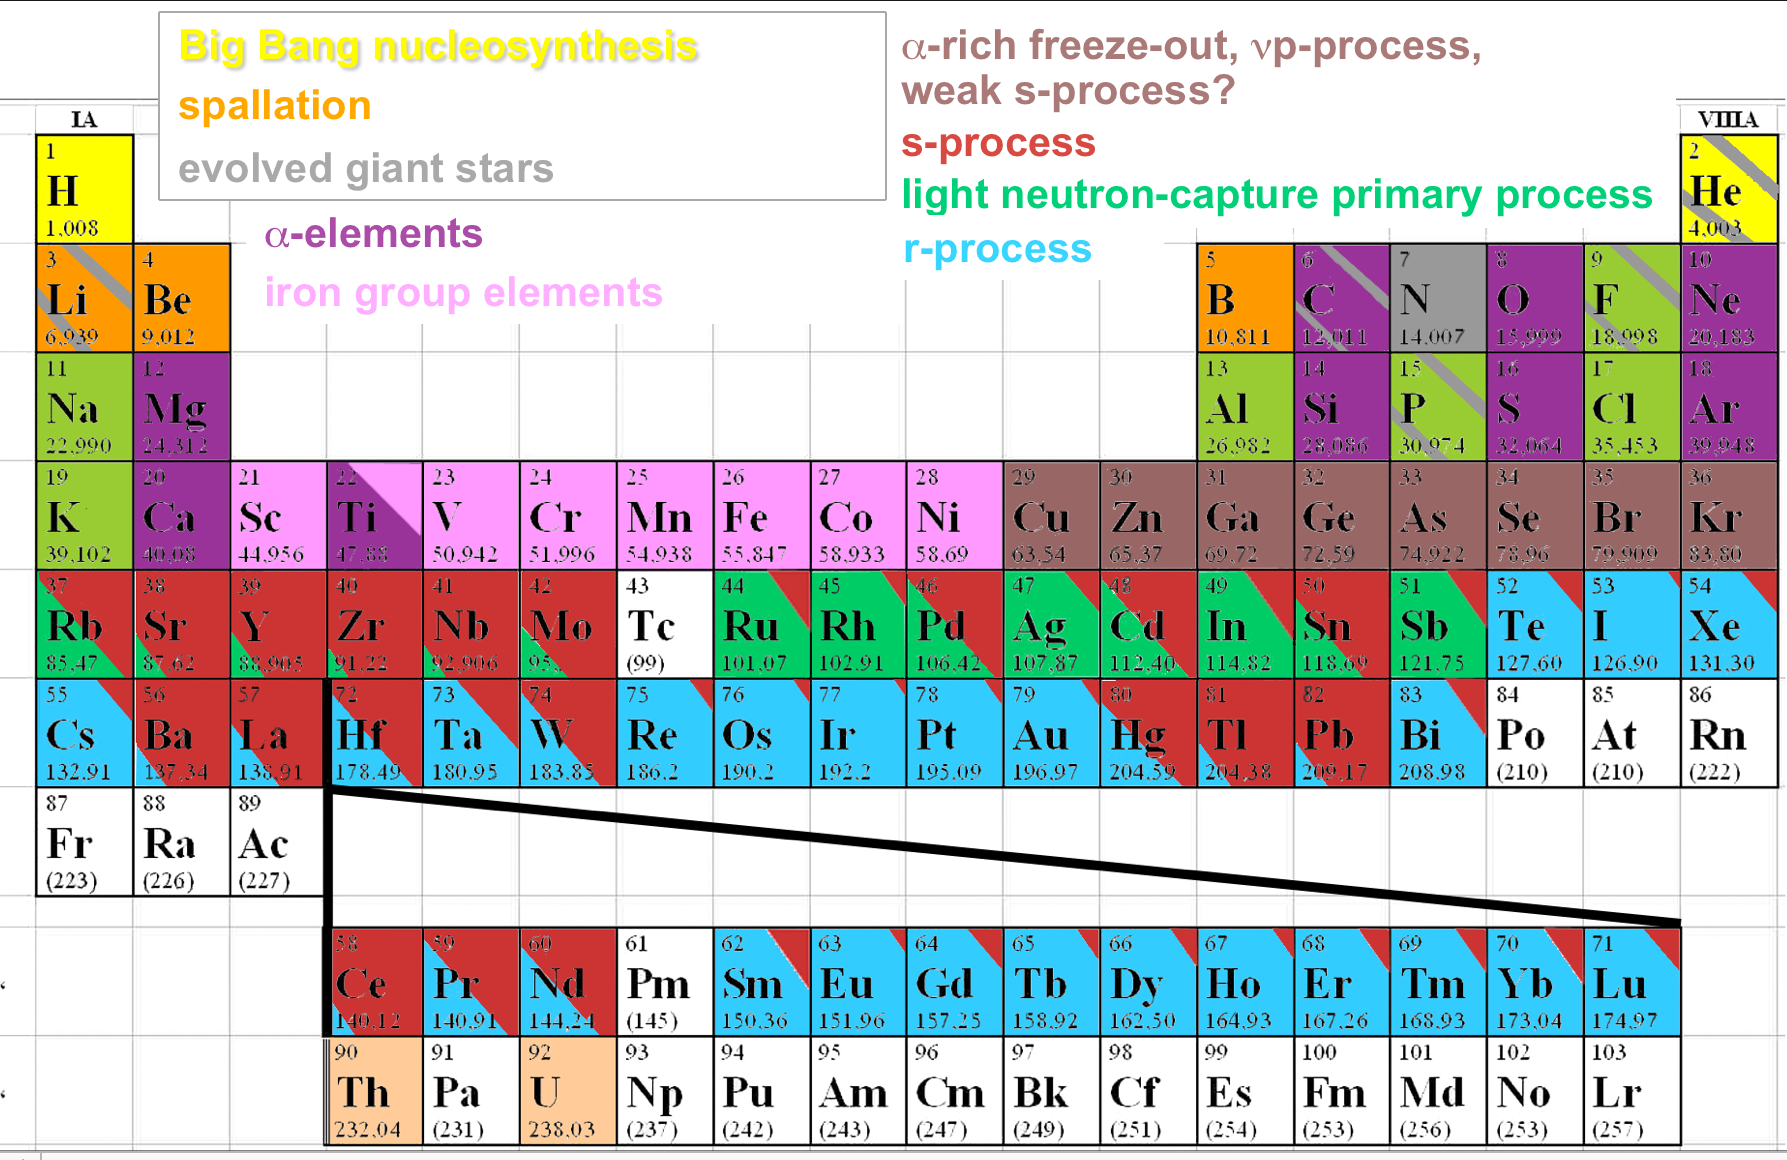
\includegraphics[width=0.75\linewidth]{./figures/intro/periodic_table}
  \caption{The periodic table of elements colored by the relative fraction of the nucleosynthetic processes that naturally occur in the Universe that produce each element. \textbf{Image Credit:} A modified version of the table created by Anna Frebel (\url{https://www.dropbox.com/sh/ib3agt2bkxqqk2u/AACbEw1warp74qzUh2AcWqfja?dl=0}), accessed on 03-18-19.}
  \label{intro:fig:periodic table}
\end{figure}

A variety of nucleosynthetic processes occur within stars and during their deaths that lead to the production of all of the elements in the periodic table. This is illustrated well in Figure~\ref{intro:fig:periodic table}, which shows the periodic table colored by the fractional importance of the nucleosynthetic processes that produce each element. Due to the diversity in production sources across the periodic table, multi-element metal abundance measurements in stars can be used to to better understand and constrain how and where each metal is produced. Exactly which reactions occur where depend strongly on the initial abundances of elements in stars, their stellar masses, and, for heavy nuclei, the neutron density.

This means that elements from different nucleosynthetic channels are produced on different timescales during a galaxy's evolution, as set by the lifetimes of the stars in which they occur, and are released into the galaxy at different energies, with different spatial distributions within the galaxy, and at different rates. For example, O, an $\alpha$-element is produced predominately in massive stars and is therefore released via core collapse supernovae on timescales of $\sim$~10~Myr after a star formation event, near their stellar birth sites. By contrast, Sr is produced predominately via the s-process (discussed more below) which occurs in part in the asymptotic giant branch (AGB) winds of lower mass stars ($M < 8$~M$_{\odot}$) at much lower energies and on timescales of $\sim 100$~Myr - $1$~Gyr. By this time, these stars would have diffused farther away from their birth sites, potentially sampling a qualitatively different portion of the ISM than the preceeding core collapse SNe. Generally, how different timescales affect observed stellar abundances patterns are well understood and easily modeled.\footnote{The canonical example of this is the ``knee" feature in a $[\alpha/$Fe] vs. [Fe/H] diagram, where the location of this knee signifies the point at which Type Ia enrichment (which produces significant Fe, but little to no $\alpha$ elements) begins to have a significant contribution over core collapse SNe (rich in $\alpha$ elements, but not Fe) \citep[e.g.[]{MatteucciBrocato1990, Geisler2005, Hill2018}. The location of this knee in this diagram shifts for a given galaxy depending on its SFH.} However, it is not well understood how differences in where and with what energies these events occur affect observed stellar abundance patterns. Investigating these differences is a key motivation of this \dissertation.

As relevant to this work, we briefly summarize a few of the important nucleosynthetic channels shown in Figure~\ref{intro:fig:periodic table} and their sites. $\alpha$-elements, notably O, Mg, Si, Ca, and Ti, are produced during the lifetime of massive stars (O, Mg) or during the core collapse supernova explosion itself. In either case, these elements are synthesized through the capture of an $\alpha$ nucleus, progressing towards increasingly heavier nuclei in intervals of 4/2 in mass/atomic number (as $\alpha$ = $^{4}_2$He) from $^8_4$Be all the way to the stable $^{52}_{26}$Fe and unstable $^{56}_{28}$Ni (which days to $^{56}_{26}$Fe). The iron group elements, notably Fe, Mn, Co, and Ni, are produced predominately in Type Ia supernovae, with variations depending on a single vs. double degenerate scenario, the initial composition of exploding white dwarf(s) (WD), and the dynamics of the explosion itself.

The presence of these heavier elements in stars enables the formation of even heavier nuclei through neutron capture. This is categorized into two processes, the slow (or s-) and rapid (or r-) process. In the former, neutron densities are typically low enough that the product of each neutron capture beta decays to a more stable isotope before capturing another nucleon. In r-process, however, the rate of neutron capture exceeds beta decay, allowing for the production of different, typically heavier, nuclei. As shown in the diagram, lighter elements are produced via the s-process and heavier via the r-process, with notable overlap in certain elements, such as Ba.\footnote{For the sake of this discussion, the light neutron-capture primary process elements (sometimes referred to as ``lighter element primary process") should be considered s-process elements. Briefly, this different nucleosynthetic channel, first identified in \cite{Travaglio2004}, arose from the disagreement between models of s-process enrichment and stellar abundances of elements including Sr, Y, and Zr. However there is still uncertainty as to whether or not these differences can be explained with different models of weak s-process (which can occur in the winds of massive stars) \citep[e.g.][]{Prantzos2018}.} The s-process occurs predominately in the low-energy winds of low mass (1-8 M$_{\odot}$) AGB stars on time scales of 100's of Myr up to 1 Gyr. Exactly which elements are produced in a given AGB star varies with stellar mass and depends strongly on metallicity, which determines the available heavy seed nuclei. Sr, Y, Zr, and Ba, as well as C, N and F, are commonly used as observational tracers of this nucleosynthetic channel.

The dominant origin of r-process enrichment is highly uncertain, though possible channels include NS-NS and neutron star - black hole mergers, neutrino driven winds in core collapse SNe, and exotic SNe, such as magnetic, jet-driven SNe, collapsars, hypernovae, and long-duration gamma-ray bursts \citep[see ][ for recent reviews]{Frebel2018, Cowan2019}. Eu is the most commonly used (and easy to observe) unambiguous observational tracer of r-process enrichment; Ba is also often studied as a tracer, but requires care due to the significant contribution from s-process enrichment. More detailed spectra \citep[e.g.][]{Ji2018a} can trace many more of these elements, which can be used as an important discriminator between nucleosynthetic models.

Finally, although the production of elements unaffected by the r-process are comparatively well understood, there are still large uncertainties in both nuclear reaction rates and stellar evolution properties that affect the computed yields for any given element. As including self-consistent nuclear reactions in the interior of stars is nearly computationally impossible in galaxy-scale simulations, metal yields are generally included as averaged over an entire stellar population (see Section\ref{intro:sec:stars}) as obtained from a tabulated set of yields. These yields for a given star in a simulation are typically IMF-averaged, and occasionally mass and metallicity dependent depending on the level of detail desired in the simulation. Often, only the global metallicity is tracked in simulations, but tracking individual metal species (especially C, O, and Si which can affect the chemistry and cooling physics in the ISM) is becoming more common. The uncertainties across tabulated yields, however, mean there are often significant variations and inconsistencies between tables produced by separate groups. These can sometimes make interpreting the results of galactic chemical evolution models challenging.

\subsection{Radiative Processes and Chemistry}
\label{intro:sec:cooling}

Radiative processes are of fundamental importance in properly modeling the diversity of density, temperature, and ionization states in a multi-phase ISM. It is via radiative cooling that gas, heated by gravitational accretion onto dark matter halos, can cool, condense, become self-gravitating, and (eventually) collapse to form stars. Conversely heating, via radiative absorption or scatterings, from stellar sources within galaxies and the extragalactic sources that comprises the cosmic UV background (UVB, e.g. \cite{HM2001,HM2012,FG2011}). Tied to both of these processes is the actual chemistry that occurs in the ISM, from the primordial chemical reactions between H, He, and free electrons to substantially more complicated reactions that occur once significant amounts of metals are present in the ISM (particularly, C, O, and Si). These metals by themselves act as additional radiative coolants, which strongly dictate the shape of the cooling curve that helps establish a multi-phase medium in the first place \citep[e.g.][]{McKeeOstriker1977}. The molecules produced in chemical reactions with these metals produce additional coolants in the ISM \citep{HollenbachMcKee1979}, including dust, which has its own rich array of associated physical processes \citep{Omukai2000,Omukai2005,Draine2011}.

A full, detailed model of radiative cooling, heating, non-equillibrium chemistry, and dust is generally far too computationally expensive to include in galaxy-scale simulations. For this reason, many large-scale cosmological simulations assume that all gas is optically thin and that all molecules and ionization states exist in equilibrium. This allows for the quick use of tabulated look-up tables for radiative cooling and heating, often produced using \code{cloudy} \citep{Cloudy2013}, that depend on gas density, temperature, metallicity, and redshift (which sets the UVB heating rate). More complex simulations often track some number (usually $< 10$) of species involved in primordial chemistry in order to better account for non-equilibrium effects and \Hmolecular production, though with noted increases in memory requirements and computational cost. Some of the most advance models to-date can account for well over 10$^2$ individual chemical reactions involving $>$ 20 elements and molecules \citep[e.g.][]{Richings2016,Richings2018}; but these are typically prohibitively expensive to run on large scales. In this \dissertation we adopt the chemistry and radiative cooling and heating physics models available in the newly developed, open-source library \code{GRACKLE} \citep{GrackleMethod}. The exact physics included in our simulations are discussed in greater detail in Chapter~\ref{ch:chapter1}, but we note that improvements to \code{GRACKLE} have been made as the direct result of the research conducted during this \dissertation.
%mention that I made improvements to this?

\subsection{Star Formation} \label{intro:sec:sf}

In galaxy-scale hydrodynamics, the costs in resolving the spatial scales and gas densities required to directly follow star formation relegates this process to a sub-grid model. Stars form from fluid elements that surpass a variety of threshold conditions at an assumed rate and efficiency. Usually, simulators set these thresholds to fully encompass gas whose Jeans-length (and thus dynamical behavior) becomes unresolved according to the widely-used \cite{Truelove1997} criterion. Often, gas is required to surpass a simple mass or number density threshold, on top of which simulators can also require that the local gas cells be in a converging flow ($\nabla \cdot \bm{v} < 0$), that gas surpass some virial threshold (describing how bound a cloud may be)
%cite?,
or that gas meet a minimum \Hmolecular mass fraction \citep[e.g.][]{Kuhlen2012}
%\citep[e.g.][]{}
. Once a fluid element is flagged as star forming, simulators have a few options to choose from in how to determine what fraction and with what rate that mass is converted into stars. Briefly, some form of the following equation is usually adopted to describe the star formation rate density,
\begin{equation}
\label{intro:eq:sfr}
 \dot{\rho}_{\rm SF} = \epsilon \frac{\rho_{\rm gas}}{t_*},
\end{equation}
where $\rho_{\rm gas}$ is the local gas density, $\epsilon$ is some fixed or variable star formation efficiency, and the timescale, $t_*$, is often adopted as the local free fall time, or
\begin{equation}
  t_* = t_{\rm ff} = \sqrt{\frac{3\pi}{32 \rm{G} \rho_{\rm gas}}}.
\end{equation}
In many cases, $\epsilon$ is fixed to some small value ($\sim$ 0.01) \citep{KrumholzTan2007} meant to represent a galaxy-scale average of star formation efficiency, even though this may vary significantly between individual molecular clouds \citep{Grudic2018}. High-resolution simulations, where the mass of stars that would form in a single time step ($dt \times \rm{SFR}$) is far less than a single star particle mass, allow stars to form out of star forming fluid elements stochastically \citep[e.g.][]{Goldbaum2015}.

Recent work has demonstrated that variations in these implementations can lead to dramatic differences in the outcome of the simulated galaxies \citep[e.g.][]{Hopkins2013,Munshi2018}. However, it is generally found that the differences between implementations decrease in simulations with sufficient resolution ($\sim$ 10~pc or better spatial, or $\sim$ $100$ M$_{\odot}$ or better in mass) and with a sufficiently high density threshold for star formation ($n > 100$~cm$^{-3}$) \citep{Orr2018,FIRE2}.

% maybe a section on each FB method? R

\subsection{Stars in Simulations} \label{intro:sec:stars}

Stars, particularly in large-scale cosmological simulations, are commonly represented as simple stellar populations (SSPs), or particles with IMF-averaged properties of stellar feedback and metal enrichment. As demonstrated in \cite{Revaz2016}, this approach is reasonable so long as the mass of the star particle is large enough to fully sample the IMF ($> 10^{4}$~M$_{\odot}$). In high resolution simulations, particularly simulations of small, low-mass systems like dwarf galaxies, this is no longer the case. This leads to inconsistencies in both the effective metal yield of the modeled stars, and (often) an artificial reduction of the effects of stellar feedback. Recent works have developed new models to address this issue, discretizing (rather than averaging over) individual feedback events \citep[e.g.][]{MUGS2010,FIRE,Hopkins2018,Rosdahl2018} or accounting for stochastic sampling of the IMF \citep{Hu2016,Hu2017,Applebaum2018,Su2018}. However, each of these methods utilizes a sub-grid recipe in some fashion to improve upon the SSPs. On the other extreme are highly resolved simulations which model star formation with ``sink particles" \citep[see for example ][]{Krumholz2004,Federrath2010,GongOstriker2013,BleulerTeyssier2014,Sormani2017} that account for the gradual accretion of gas in the growth of a single star (or group of stars) and protostellar feedback. These recipes are often computationally expensive, however, restricting their use over long timescales (100's to 1000's of Myr or more) in galaxy-scale simulations.

In this \dissertation, we develop the first implementation that breaks the SSP formalism entirely by following stars as individual star particles sampled from an adopted IMF. This allows us to place unprecedented detail on both the stellar feedback and metal yields associated with each star, spatially and temporally resolving differences in both of these channels as a function of stellar mass and metallicity.

\subsection{Stellar Feedback} \label{intro:sec:feedback}

The first models of galactic evolution produced galaxies with stellar masses far in excess of what is observed in the Universe.
%, converting a substantial fraction of their baryons into stars.
From these initial works, it was clear that some form of feedback process must take place to self-regulate star formation within galaxies. With observations of metal abundances in the CGM around galaxies \citep[see][ for a recent review]{Tumlinson2017}, and of fast-moving outflows from star forming galaxies \citep[see][ for a review]{Veilleux2005}, it was additionally clear that some mechanism must exist to drive these outflows. Stellar feedback became the clear physical mechanism to account for both of these phenomena.\footnote{Except maybe for more massive galaxies, where active galactic nuclei may play some role in regulating star formation and certainly play a role in driving outflows \citep[e.g.][]{Fabian2012}. We do not discuss this source of feedback further in this \dissertation aside from noting that it is another significant uncertainty in our understanding of galactic evolution.}

Initial models for stellar feedback relied primarily on the energy injection from supernovae (SNe, see Section~\ref{intro:sec:supernovae}) to regulate star formation and drive outflows, but it has become clear that this mechanism alone cannot completely account for all of the star formation, ISM, outflow, CGM, and even intergalactic medium (IGM) properties of observed galaxies (see \cite{SomervilleDave2015} and \cite{NaabOstriker2017} for recent reviews and more detailed discussion of how feedback impacts outstanding problems in galactic evolution). Other sources of effective stellar feedback have been identified since \citep[e.g.][]{Agertz2013}, which serve to regulate star formation on different timescales and help develop and ISM and CGM with different phase and ionization properties. This includes both stellar radiation (Section~\ref{intro:sec:radiation}) and stellar winds (Section~\ref{intro:sec:stellarwinds}).

Although not included in this \dissertation, for the sake of completeness, we mention a few additional sources of stellar feedback that likely contribute to the full picture of galactic evolution. A substantial amount of recent research has been dedicated towards the examination of supernova-driven cosmic ray feedback (see Section~\ref{ch1:sec:CRs} for a more detailed discussion and references). In brief, cosmic rays can be a dominant source of heating in very dense gas and act as a source of non-thermal pressure in the ISM, which can drive galactic winds with qualitatively different phase structures \citep[e.g.][]{SalemBryanCorlies}. Binarity is often ignored in models of stellar feedback. The effects of binary evolution can dramatically extend the timescales over which ionizing radiation and supernovae act in a newly formed stellar populations. Typically, this increases their total energy output and decreases the ISM densities in which SNe explode, increasing their effectiveness (see Section~\ref{ch1:sec:binary stars}). Finally, exotic sources of stellar feedback, such as hypernovae, high-mass X-ray binaries, and NS-NS mergers can also be a potentially important sources of feedback, particularly in the lowest mass halos \citep[e.g.][]{Artale2015}. However, the uncertainties in the frequency and delay time distributions for when these events should occur, and their relative rarity, preclude including these effects in this \dissertation.

\subsubsection{Supernova Feedback}
\label{intro:sec:supernovae}

In the simplest model, supernova feedback is treated as the injection of pure thermal energy (and mass) into the fluid element(s) that are host / closest to the chosen site of a supernova explosion. In self-consistent models of star formation and feedback these sites are usually actual star particles, but this does not have to be the case. The first models which included supernova feedback lacked the spatial / mass resolution to resolve individual (or even collective) SN events. This is the source of the commonly known ``overcooling" problem, whereby too little energy is injected into too much mass such that the affected region only reaches modest temperatures ($T \lesssim 10^5$~K, as opposed to $T > 10^7$~K, or so). This temperature is right around the peak of the cooling curve, and thus the energy is rapidly radiated away before it has time to make a significant dynamical impact of the galaxy. This is still a problem today in large-box simulations of cosmological volumes which have insufficient resolution to resolve individual SNe. While some of the initial, ad-hoc fixes for this problem (e.g. turning off cooling for some time in SN affected fluid elements or decoupling SN affected SPH particles from the hydrodynamics for some time) are still in use today, some notable advancements have been made to employ some combination of kinetic, momentum, and thermal energy feedback to attempt to capture SNe in a more consistent fashion \citep[e.g.][]{FIRE,Simpson2015,Hopkins2018}.

High resolution simulations, like those developed in this \dissertation, can typically rely on using pure thermal energy injection while still avoiding artificial overcooling.\footnote{This is advantageous because it is often substantially easier to implement than kinetic / momentum injection methods while being less susceptible to numerical artifacts, especially for grid-based codes.} This is true for simulations with typical spatial / mass resolutions better than a few pc / 10 M$_{\odot}$ \citep{Simpson2015,Hu2018,Smith2018b}. However, a spatial resolution requirement is a density dependent statement; in this case supernovae that occur in the densest gas ($n > 10^{2-3}$~cm$^{-3}$) may still be under-resolved and ineffective. In this case, accounting for feedback processes from massive stars that occur before the first core collapse SN in a given star formation event becomes critical \citep{Hu2016}. Including these physics, as discussed below, greatly reduces the typical ISM densities in which SNe occur, greatly increasing the likelihood that these events are well resolved.

\subsubsection{Stellar Radiation}
\label{intro:sec:radiation}

We only briefly discuss this method of feedback here, as it is discussed in much more detail in both Chapters~\ref{ch:chapter1} and \ref{ch:chapter2}. In brief, \cite{Leitherer1999}, \cite{Agertz2013}, and others have demonstrated that stellar radiation accounts for a substantial fraction of the total energy output of a stellar population. Ionizing photons from young, massive stars can photoionize and heat the gas surrounding sites of recent star formation. This pre-processes the local environment within which SNe occur, often increasing the effectiveness of SNe in regulating star formation and driving outflows \citep{Hu2016}. In addition, radiation pressure in the single-scattering limit (from UV photons) and rescattered infrared photons has been used as an additional source of pre-SN feedback \citep[e.g.][]{FIRE}. However, due in part to differences in how ionizing radiation is followed across simulations, there is disagreement as to exactly how and in what conditions this acts as a source of feedback (see \cite{Krumholz2018} for a detailed examination of this problem).

Non-ionizing radiation also contributes to the regulation of star formation and the multi-phase ISM. Far ultraviolet (FUV) photons contribute to gas heating via the photoelectric heating of dust grains. This is a significant heating mechanism in higher metallicity environments, like the Milky Way \citep{Parravano2003,Wolfire2003}, but may still be important in setting temperature floor of cold dense gas in lower mass galaxies \citep{Forbes2016,Hu2017}. Lyman-Werner (LW) band radiation regulates the \Hmolecular~ abundance, which is particularly important in low-metallicity environments where \Hmolecular~ is a dominant coolant \citep[e.g.][]{Glover2003,Wolcott-Green2012}.\footnote{And is arguably even more important when using star formation perscriptions that depend upon the local \Hmolecular mass fraction.} As the goal of this \dissertation is to develop an as-complete-as-possible model of galactic chemical evolution, we account for each of these processes in some fashion.

The simplest way to model stellar radiation feedback is to apply an optically thin, analytic radiation profile, such as the galaxy-centered exponential photoelectric heating profile used in \cite{Tasker2009}, or $1/r^2$ profiles from individual sources \citep[e.g.][]{Forbes2016}. However, radiative transfer effects, such as gas self-shielding, are often important, particularly for ionizing radiation. Solving the equations of radiative transfer directly in simulations -- as is done with ray tracing methods -- is computationally expensive and scales significantly with the number of sources. For this reason, approximate methods, such as flux-limited diffusion, treat radiation as a fluid, removing the scaling of computational cost with the number of sources. In this \dissertation, we follow the evolution of galaxies that have at most $10 - 100$ ionizing sources at one time, making it computationally feasible to use the accurate adaptive ray-tracing radiative transfer method implemented in \code{Enzo}.

\subsubsection{Stellar Winds}
\label{intro:sec:stellarwinds}

Stellar winds, in addition to stellar radiation, are a potentially important source of pre-SN feedback that helps regulate star formation in / around the birth clouds of newly formed stars. However, the hot ($T>10^{6}$~K), fast ($v \sim 10^{3}$~km~s$^{-1}$) winds from massive stars \citep{Weaver1977} are challenging to model self-consistently in galaxy-scale simulations. For this reason, there has been comparatively little research on how they affect global galaxy properties, even though some models do include their energy injection in an integrated / approximate fashion \citep[e.g.][]{FIRE}. However, stellar winds, from both massive stars and weaker winds from the AGB phase of low mass stars, are important sources of metal enrichment. For this reason we include stellar wind feedback in this \dissertation, albeit in a simplified fashion.\footnote{Although we do not have conclusive results to this end, initial examination of our simulations has shown that our stellar wind model is only globally important in simulations where radiation feedback is ignored. It is thus likely sub-dominant to radiation feedback.}

\section{Observations of Local Group Dwarf Galaxies}
\label{intro:sec:LG dwarfs}

We are motivated by using a properly formed model for galactic chemical evolution in dwarf galaxies to interpret and explain observations of Local Group dwarfs. As any good theoretical work should maintain a close connection to the observations that motivate the study in the first place in order to better make predictions for future observations, we devote some time here to summarize relevant observations of Local Group dwarfs.

\subsection{Known Dwarf Galaxies of the Local Group}
\label{intro:sec:dwarf galaxies}

The Milky Way and its local environment is host to a diverse collection of dwarf galaxies. The properties of these galaxies have been nicely summarized in a recent review \citep{Tolstoy2009}, and again in \cite{McConnachie2012}. However, the number of known Local Group dwarf galaxies has increased dramatically since that time, particularly for the Milky Way, whose known satellite population has more than doubled. This is due in large part to tremendous improvements in our ability to detect galaxies on the faintest end of the luminosity function, called ultrafaint dwarf galaxies \citep[UFDs][]{Willman2005}.\footnote{See \cite{Simon2019} for a recent review}. The Dark Energy Survey \citep[e.g.][]{Drlica-Wagner2015} and Hyper Supbrime-Cam \citep[e.g.][]{Greco2018} have made tremendous advances to this end, with the upcoming Large Synoptic Survey Telescope expected to produce an even greater increase in the known population of faint galaxies in the Local Group \citep{Haynes2019,Weisz2019}.

While there is no true sharp transition below which a galaxy is considered ``dwarf", historical definitions are based on luminosity cuts, using the SMC and LMC as rough anchor points for the upper-end of the dwarf galaxy scale. \cite{Bullock2017} suggests a delineation based on stellar mass. For this \dissertation, we follow this definition and consider galaxies with $M_* < 10^9$~M$_{\odot}$ as dwarf galaxies, and galaxies with $M_* < 10^5$~M$_{\odot}$ as UFDs. In general, dwarf galaxies are extremely dark matter dominated, with mass to light ratios over 10$^2$ \citep{SimonGeha2007,Strigari2008,Wolf2010}, convert gas into stars at a lower efficiency than more massive galaxies (cite), and, for the lowest mass dwarf galaxies
% need citations
, exhibit bursty star formation histories driven by stochasticity in the process of both star formation and the effects of stellar feedback
% need citations
.

\subsection{Metals in Local Group Dwarfs}
\label{intro:sec:metals in LG}

The first studies of stellar abundances in the Local Group focused on stars in nearby dwarf spheroidals (dSph's), and massive stars in the LMC, SMC, and similar, more massive dwarf galaxies. These studies typically obtained abundances for only a small sample ($\sim$ 10) stars, limiting the extent to which they can be used to test models of galactic chemical evolution.  However, the advent of high-resolution spectrographs at both Keck and the Very Large Telescope -- capable of obtaining the spectra of many stars with a single pointing -- have dramatically increased the sample size of stellar abundances in nearby dwarf galaxies.

Stellar feedback drives outflows, galactic winds, from galaxies across all scales
%(references).
Dwarf galaxies in particular, with their relatively shallow potential wells, are expected to drive effective galactic winds \citep{MacLowFerrara1999} with mass loading factors ($\eta$ = $\dot{\rm{M}}_{\rm out} / {\rm SFR}$) above 100 \citep{Muratov2015,Christensen2018}. Not only does this correspond to a significant amount of mass outflow from these galaxies, but these winds should also carry out a substantial amount of metals from these galaxies. In fact, the differences with which different models for feedback-driven winds drive metals in outflows in low mass galaxies can be an important constrain on the underlying physics \citep[e.g.]{Wheeler2018,Agertz2019}. \cite{Kirby2011-metals} used measurements of the stellar abundances in Local Group dSph's and their resolved star formation histories to determine that their stars contain less than 5\% of the metals synthesized in each galaxy. However, since these galaxies have lost their gas through environmental processes as satellites of the Milky Way (primarily ram pressure and tidal stripping), it was unclear if this loss could be attributed entirely to feedback. However, using gas and stellar abundances \cite{McQuinn2015} showed that Leo P -- a gas-rich Local Group dwarf galaxy -- has also ejected $\sim$95\% of its metals (see Section~\ref{intro:sec:Leo P}). This is significant evidence for metal-enriched, feedback-driven galactic winds operating in these low mass dwarf galaxies.

Finally, the low metallicities of the lowest mass dwarf galaxies make them ideal places to better constrain large uncertainties in stellar nucleosynthesis \citep{FrebelNorris2015,Frebel2018}. At these low metallicities, the number of possible enrichment events that could have possibly contributed to the observed stellar abundances decreases significantly, increasing the possibility of using these abundance patterns to constrain the yields of individual sources. This is particularly true for exotic enrichment events, like those expected to be sources of r-process elements, which are potentially so rare that only one or fewer events would be expected in an individual low-mass galaxy.

The most prominent example of these types of studies has been of the UFD Reticulum II, where \cite{Ji2016} used the extreme r-process enhancement in its stars to argue in favor of a NS-NS of r-process enrichment. This conclusion has been supported by observations in additional Local Group dwarf galaxies \citep{Duggan2018}, but there is still some disagreement as to the dominant source of r-process enrichment \citep[e.g.][]{Siegel2018}. Interestingly, the lack of these extreme r-process abundances in other UFDs suggests that another source of r-process must exist \citep{Ji2016b}. Some of the significant uncertainties in interpreting these observations lie with understanding how r-process elements mix within the ISM and are ejected from low mass dwarf galaxies. Recent research has examined how metals from individual enrichment events may mix and evolve in a variety of contexts \citep[e.g.][]{Bland-Hawthorn2015,Ritter2015,Montes2016,Safarzadeh2017}, but there is still much to be understood about this process. In particular, there is still much to be gained from adapting insights from these types of simulations to the modeling used to interpret observations of stellar abundances (as discussed in more detail in Section~\ref{intro:sec:onezone}).

\subsection{Leo P: A Case Study}
\label{intro:sec:Leo P}

\begin{figure}
 \centering
 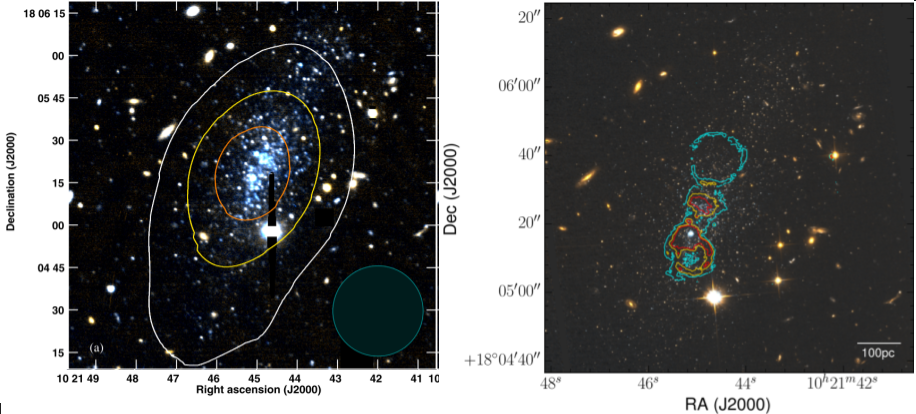
\includegraphics[width=0.975\linewidth]{figures/intro/Leo_P}
 \caption{The Leo P dwarf galaxy. \textbf{Left:} \hi contours from the Very Large Array (VLA) at 32'' resolution overlaid on top of an optical Large Binocular Telescope image. 32'' is the lowest resolution \hi observation available of Leo P from the VLA, which best traces diffuse, warm ($T \sim 10^3$~K) \hi in the galaxy and exhibits the full spatial extent of its gas content. This image is adopted from the top-left panel of Figure 4 in \cite{Bernstein-Cooper2014}. \textbf{Right:} H$\alpha$ emission (contours) overlaid on top of a Hubble Space Telescope (HST) optical image. The \hii region analyzed in \cite{McQuinn2015} to obtain gas-phase metallicities is the blue clump of H$\alpha$ towards the bottom of the image. This image is adopted from Figure 10 of \cite{Evans2019}. Note the inversion in the vertical axes between the left and right panels.}
 \label{intro:fig:Leo P}
\end{figure}

We dedicate this section to a specific Local Group dwarf galaxy, Leo P, as its observed properties motivate the initial conditions of the simulations developed in this \dissertation. This galaxy is remarkable for being one of the lowest mass dwarf galaxies with observed, ongoing star formation. It is located at a distance of $1.62\pm 0.15$~Mpc \citep{McQuinn2015a}, and was first characterized as part of the ALFALFA survey \citep{Giovanelli2013,Rhode2013,Skillman2013,McQuinn2013,Bernstein-Cooper2014}. These studies have characterized its star formation history as low and roughly continuous over the age of the Universe \citep[$<$SFR$>$ = $4.3\times 10^{-5}$~M$_{\odot}$~yr$^{-1}$,][]{McQuinn2015a}, its stellar mass \citep[$M_{*} = 5.7 \times 10^{5}$~M$_{\odot}$,][]{McQuinn2013}, its \hi and dynamical mass \citep[$M_{\rm HI}(r<r_{\rm HI}) = 9.5\times 10^{5}$~M$_{\odot}$, $M_{\rm dyn}(r<r_{\rm HI}) = 2.6 \times 10^{7}$~M$_{\odot}$, $r_{\rm HI} \sim 500$~pc,][]{Bernstein-Cooper2014}, and gas-phase abundances from an \hii region \citep[12 + log(O/H) = 7.17$\pm$0.04][]{Skillman2013}. HI, optical, and H$\alpha$ observations of Leo P are shown inf Figure~\ref{intro:fig:Leo P}.

We chose to focus on a Leo P like galaxy in our simulations in part to allow for comparisons to the work in \cite{McQuinn2015}, which makes an accounting of the total metals (as traced by O) contained in the ISM and stars in Leo P, estimating the fraction that must have been ejected over the lifetime of the galaxy.
%This is an important measurement as prior estimates of this number for low mass dwarf galaxies were restricted to Milky Way dSph's, which are devoid of gas and contaminated by environmental affects.
As of this writing, Leo P is one of the only low mass dwarf galaxies with both gas-phase and stellar metal abundance measurements, but there is ongoing work to greatly expand this sample in the near future.

\section{Onezone Models of Galactic Chemical Evolution}
\label{intro:sec:onezone}

This \dissertation utilizes high-resolution hydrodynamics simulations that are expensive to run in terms of both wall-time ($\sim$ weeks to months) and computational time ($\sim 10^{5-6}$ CPU hours). For this reason, it is computationally infeasible to directly explore many of the uncertainties associated with each of the components of the model as discussed in Section~\ref{intro:sec:ingredients}. For this reason, substantially cheaper semi-analytic models are valuable tools that can be used to better understand galactic evolution.

One of the most common ways to model and understand the stellar populations of galaxies in high-dimensional chemical space is through simplified one-zone (or many-zone) models. This treatment extends back many decades \citep[e.g.][]{Schmidt1963,TalbotArnett1971,Lynden-Bell1975}, where galaxies and their total metal abundances were treated in closed-box systems of gas and stars. Over the intervening decades these models have improved, including prescriptions for gas outflow (a ``leaky-box") or gas inflow (an ``accreting box"), or both \citep[a ``bathtub" model, e.g.][]{FinlatorDave2008,Bouche2010}. The assumptions that go into these models vary dramatically with complexity. Simple models can assume, for example, that long-lived low mass stars do not contribute to metal enrichment while metals from massive stars are instantaneously recycled into the galaxy's gas reservoir (i.e. ignoring stellar lifetimes) or that all metals mix instantly and homogeneously. More complex models account for individual stellar lifetimes (to some degree), or may try and account for some aspects of inhomogeneous mixing by constructing multi-zone models that may separate a galaxy in radial bins (with or without mixing between bins), may account for a hot and cold component separately (with mixing between the two), or account for separate ISM and CGM components. The output of these models is typically the mean metal abundance evolution within each of the tracked components. There is generally no self-consistent prescription to account for the scatter in any abundance relationship in these models, which, when needed, is often added ad-hoc in post-processing. Regardless of the assumptions that go into these models, they are powerful tools that can be used to probe the general physical processes that govern galactic chemical evolution, and explore the vast, uncertain parameter space associated with the models that characterize these processes \citep[e.g.][]{Cote2017a}.

One final motivation of this \dissertation is to improve the assumptions within these models by better characterizing the process of inhomogeneous mixing in the ISM, and the coupling of metals to galactic winds and outflows. This is particularly important if the behavior differs between elements from different nucleosynthetic sites. In addition, this work could be used to account for the spread and higher-order statistics of stellar abundance distributions, which would be a powerful tool for better leveraging the wealth of observations in the Milky Way and Local Group. Yet, as discussed, the current state of the art prescriptions for these processes are ad-hoc. Recent analytic work in \cite{KrumholzTing2018} lays down a framework to evaluate the correlation between individual metals in different galactic environments and predicts that the correlations will differ for different nucleosynthetic sites (e.g. AGB winds vs. SNe). We characterize these differences in detail in Chapter~\ref{ch:chapter3}, laying the groundwork for how one could potentially incorporate this insight into improving these models. We build upon this idea more in Chapter~\ref{ch:chapter4}, and plan to explore the connection between our simulations and analytic models in the future. Recent work by \cite{SchonrichWeinberg2019} is a great example of how this could impact current models for galactic chemical evolution. The authors show how adopting a two-phase model (hot and cold ISM), along with parameters for how metals are injected and mix between the phases whose values differ depending on nucleosynthetic origin of the metal, can reconcile long-standing problems in understanding the r-process abundance evolution of stars in the Milky Way. In fact, they argue that it would be impossible to reproduce observed r-process abundances in the Milky Way (namely [Eu/Fe], [Eu/Si], and [Eu/Mg] as functions of [Fe/H]) with a standard one-phase model.


\section{Structure of \dissertation}\label{intro:sec:structure}
\label{intro:sec:structure}

In this work we investigate the role of both stellar feedback and mixing in a multi-phase ISM in driving galactic chemical evolution. Using a novel method for following star formation and stellar feedback in galaxy-scale hydrodynamics simulations, we provide significant insight into how individual metals from distinct nucleosynthetic sites enrich the ISM, how their abundances are set and imprinted upon newly formed stars, and how they are ejected from galaxies through galactic winds.

In Chapter \ref{ch:chapter1} \citep[published as][]{Emerick2019}, we motivate the need for a new model of star formation and stellar feedback to address the open uncertainties in galactic chemical evolution. We implement such a model, which follows stars as individual star particles over a fully sampled IMF, in hydrodynamics simulations of an isolated, low-mass dwarf galaxy. We describe in detail the physics included in these simulations, including a stellar feedback model that follows stellar radiation, stellar winds, and supernovae. We find that the implemented set of physics give rise to a multi-phase ISM with a highly variable stellar radiation profiles, star formation rates, and galactic outflows. In agreement with previous works, we find that multi-channel feedback is able to drive outflows with high mass-loading factors while maintaining a fluctuating star formation rate density consistent with observations of low mass dwarf galaxies. Finally, we characterize the \Hmolecular~ properties of this galaxy, which remains unconstrained in observations of dwarf galaxies at this mass scale.

In Chapter \ref{ch:chapter2} \citep[published as][]{Emerick2018a}, we investigate how stellar ionizing radiation feedback impacts the evolution of our simulated low mass dwarf galaxy. We confirm the findings in recent works, as discussed in Section~\ref{intro:sec:radiation}, that find that stellar radiation is an important source of pre-supernova feedback that regulates star formation and can help drive galactic outflows. We additionally investigate how radiation feedback couples to the ISM to drive galactic winds by demonstrating that the ionization of gas far from individual ionizing sources, out into the disk-halo interface of our galaxy, creates low-density channels through which supernovae can readily drive gas and metals into and beyond the galaxy's CGM. This suggests that not only is the local deposition of energy from stellar radiation important, which quickly destroys dense gas in stellar birth-sites, but also long-range effects are important to consider in a consistent model of stellar feedback.

In Chapter \ref{ch:chapter3} \citep[published as][]{Emerick2018b}, we dive in detail into the evolution of each of the 15 individual metal species that we follow in our simulation. We focus primarily on the evolution of the gas-phase abundances of these metals, and how the site of nucleosynthesis (e.g. AGB winds or SNe) drives the subsequent evolution of each species. We find that elements released in lower energy enrichment sources (e.g. AGB winds) mix less effectively in the ISM across all phases than elements released in higher energy enrichment sources (e.g. SNe). Likewise, energy differences associated with their enrichment directly impacts their ability to couple to galactic outflows. We find that elements released in AGB winds are retained at a higher fraction (by a factor of $\sim$ 4-5) than elements released in SNe.

In Chapter \ref{ch:chapter4} we discuss recent, unpublished results which build upon the work in Chapter~\ref{ch:chapter3} by investigating in more detail how energy, spatial location within the galaxy, and galaxy SFR affect the mixing and ejection of metals for individual enrichment events. With a more detailed study, we again confirm that metal mixing in the ISM and ejection in galactic winds depends upon the energy of the enrichment event, sampling event energies from AGB winds ($\sim$ erg) to hypernovae ($\sim 10^{52}$~erg).

Finally, we conclude in Chapter \ref{ch:conclusion} and briefly discuss future work as extensions of this \dissertation.
